\documentclass[
    size=20pt,
    style=sailor,
    display=slides,
    paper=smartboard,
    orient=landscape,
]{powerdot}

\pdsetup{
    logohook=bl,
    logopos={0.04\slidewidth,0.02\slideheight},
    logocmd={\includegraphics[height=0.12\slideheight]%
    {../common_figures/DTU_orig.eps} } ,
    trans=Wipe,
    palette=Wine,
}
\usepackage{../common_packages/powerdot_presentation}
% Nice minted tutorial
% https://www.sharelatex.com/learn/Code_Highlighting_with_minted
\usepackage{minted}
\newminted{python}{fontsize=\footnotesize}

% Presentation metadata
\title{The python debugger}
\author{Michael L{\o}iten\\
\texttt{mmag@fysik.dtu.dk}\\
Slides and programs:
\href{https://github.com/loeiten/python_club/tree/master/15.04.29-pdb_debugger}{
\texttt{github.com/loeiten/python\_club}} }
\date{\today}

\begin{document}
\maketitle

%  Example 
%  n(ext)
%  s(tep)
%  unt(il) [lineno]
%  r(eturn)
%  c(ont(inue))
%  j(ump) lineno
%  l(ist) [first[, last]]
%  ll | longlist
%  a(rgs)
%  p expression

% Example
% import pdb
% import my_debug_example_fail
% my_debug_example_fail.main()
% ...
% pdb.pm()
% Post mortem the failed file, and change a_list to a list
% show the help
% (pdb)b="bbb"
% Up, down
%
% Change to something that works
% python -m pdb my_debug_example.py
% Set new condition for the bp (demo) -> if i==3
% b 40, i==1
% Breakpoint in the for loop commands 1 -> (com) p i
% commands 1
% (com) p 'hey'
% (com) end
% display i
% alias (demo) foo print('hello'))







\begin{slide}{pdb}
\vspace*{4cm}
\begin{center}
 \textbf{p}ython \textbf{d}e\textbf{b}ugger\\
 An elegant way to debug (find mistakes in) your python code
\end{center}
\end{slide}




% section: title takes up full slide
\section{Short intro to the stack frame}

\begin{slide}[method=file]{Stack-frame}
 What is all this stack-frame fuzz? (freely after 
\href{www.cs.swarthmore.edu/~richardw/cs21-s12/stack-example.pdf}{
\texttt{this reference}})
 \inputminted[fontsize=\scriptsize, linenos]{python}{programs/stack_example.py}
 \vspace*{-6cm}
   \begin{figure}[h!tb]
    \onslide{2}{
    \hspace*{10cm}
    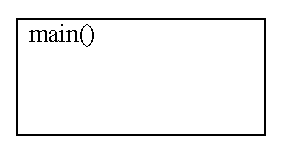
\includegraphics[width=0.30\linewidth]{figures/stack1}
    }
    \vspace{-3cm}
    \onslide{3}{
    \hspace*{10cm}
    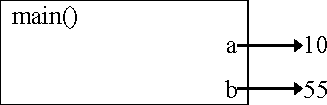
\includegraphics[width=0.30\linewidth]{figures/stack2}
    }
    \vspace{-1.5cm}
    \onslide{4}{
    \hspace*{10cm}
    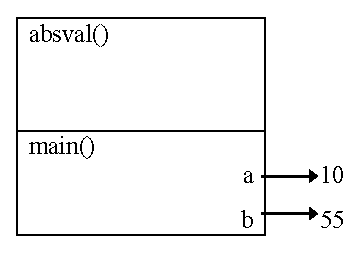
\includegraphics[width=0.30\linewidth]{figures/stack3}
    }
    \vspace{-4cm}
    \onslide{5}{
    \hspace*{10cm}
    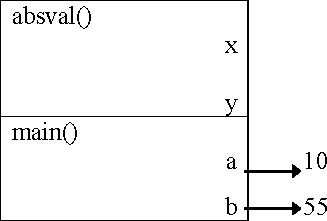
\includegraphics[width=0.30\linewidth]{figures/stack4}
    }
    \vspace{-4cm}
    \onslide{6}{
    \hspace*{10cm}
    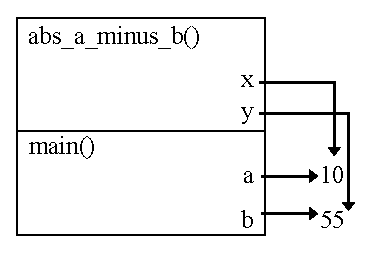
\includegraphics[width=0.30\linewidth]{figures/stack5}
    }
    \vspace{-4cm}
    \onslide{7}{
    \hspace*{10cm}
    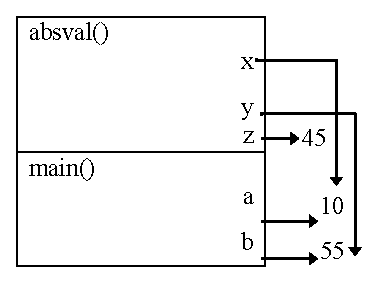
\includegraphics[width=0.30\linewidth]{figures/stack6}
    }
    \vspace{-4cm}
    \onslide{8}{
    \hspace*{10cm}
    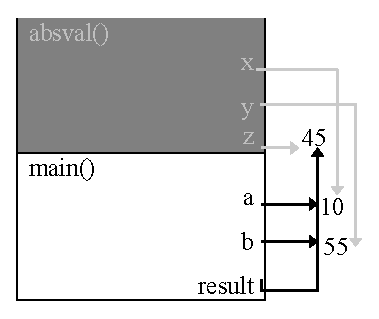
\includegraphics[width=0.30\linewidth]{figures/stack7}
    }
   \end{figure}
 \onslide{9}{
 The \textbf{traceback} prints the stack trace
 }
\end{slide}


\section{Executing pdb}


\begin{slide}[method=file]{Starting the debugger}
   \begin{minted}[fontsize=\footnotesize]{python}
# From command line
python -m pdb my_debug_example.py

# Running script
import pdb
pdb.set_trace()

# In interpreter
import pdb
import my_debug_example
pdb.run('my_debug_example.main()')


# Post-mortem
>>> import pdb
>>> import my_debug_example_fail
>>> my_debug_example_fail.main()
...
>>> pdb.pm()

  \end{minted}
\end{slide}


\begin{slide}[method=file]{Post mortem running as script}
\href{http://stackoverflow.com/questions/242485/starting-python-debugger-automatically-on-error}{
\texttt{Source}}
   \begin{minted}[fontsize=\footnotesize, linenos]{python}
import pdb, traceback, sys

def bombs():
    a = []
    print a[0]

if __name__ == '__main__':
    try:
        bombs()
    except:
        type, value, tb = sys.exc_info()
        traceback.print_exc()
        pdb.post_mortem(tb)
  \end{minted}
\end{slide}


\begin{slide}[method=file]{Executing commands}
\vspace{\stretch{1}}
\begin{minted}[fontsize=\footnotesize]{python}
# Execute the statement
pdb.run(statement, globals=None, locals=None)

# As above, and returns the value of the expression
pdb.runeval(expression, globals=None, locals=None)

# Call a function
pdb.runcall(function, *args, **kwds)

# Hardcode a breakpoint
pdb.set_trace()

# Enter debugger at post mortem given the traceback
#if none is given it takes the current exception
pdb.post_mortem(traceback=None)

# Enters pdb of last found traceback
pdb.pm()

# Can also do all of this manually by
pdb.Pdb(completekey='tab', stdin=None, stdout=None, skip=None, nosigint=False)
\end{minted}
\vspace{\stretch{1}}
\end{slide}


\section{pdb commands}

\begin{slide}[method=file]{Often used commands 1}
\vspace{\stretch{1}}
\begin{minted}[fontsize=\footnotesize]{python}
# Step into first possible occasion (can step into functions)
s(tep)

# Go to next line of expression
n(ext)

# Execute until lineno OR end of frame OR to a greater line than the current
# Convenient in for loops
unt(il) [lineno]

# Continue until function returns
r(eturn)

# Continue, only stop if bp is hit
c(ont(inue))
\end{minted}
\vspace{\stretch{1}}
\end{slide}


\begin{slide}[method=file]{Often used commands 2}
\vspace{\stretch{1}}
\begin{minted}[fontsize=\scriptsize]{python}
# Set next line to be executed (at the bottom most frame)
# Jump back and execute code again or skip part of code
# (Not always allowed)
j(ump) lineno

# List the source code around current line
l(ist) [first[, last]]

# List source for current function or frame
ll | longlist

# Print arguments of current function
a(rgs)

# Evaluate the expression, and print its value
# Similar to print(), but print() is a python function
p expression

# The same as above, but with prettyprinted function
pp expression

# Empty line: Previous command is repeated
#
\end{minted}
\vspace{\stretch{1}}
\end{slide}



\begin{slide}[method=file]{Demonstration}
Play around with \texttt{programs/my\_debug\_example.py} file if you are at 
home, not attending the presentation
\vspace{\stretch{1}}
\inputminted[fontsize=\footnotesize, linenos, firstline=1, 
lastline=12]{python}{programs/my_debug_example.py}
\vspace{\stretch{1}}
\end{slide}


\begin{slide}[method=file]{More commands}
\vspace{\stretch{1}}
\begin{minted}[fontsize=\scriptsize]{python}
# Help and documentation
h(elp) [command]

# Print the stac trace (recent frame in bottom)
w(here)

# Move frames
d(own) [count]
u(p) [count]

# W/o arguments: List the breakpoints
# Make a breakpoint (where the debugger will stop)
# Honor the breakpoint if condition evaluates true
b(reak) [([filename:]lineno | function) [, condition]]

# Temporary breakpoint (removed when hit)
tbreak [([filename:]lineno | function) [, condition]]

# Clear breakpoints
cl(ear) [filename:lineno | bpnumber [bpnumber ...]]

# Disable breakpoints (can be re-enabled)
disable [bpnumber [bpnumber ...]]

\end{minted}
\vspace{\stretch{1}}
\end{slide}


\begin{slide}[method=file]{Even more functions}
\vspace{\stretch{1}}
\begin{minted}[fontsize=\scriptsize]{python}
# Enable bp number
enable [bpnumber [bpnumber ...]]

# Ignore bp count times (if cout>0)
ignore bpnumber [count]

# Set new condition for the bp
condition bpnumber [condition]

# Specify commands for bpnumber (or the last)
# end ends the command
# silent disables info about bp reached
commands [bpnumber]

# Print type of expression
whatis expression

# Try to get the source for the given object
source expression

# Stop and display the value of the expression if changed
# Somewhat similar to watchpoints in gdb
display [expression]

# Stop displaying in current frame
undisplay [expression]
\end{minted}
\vspace{\stretch{1}}
\end{slide}


\begin{slide}[method=file]{Last functions}
\vspace{\stretch{1}}
\begin{minted}[fontsize=\scriptsize]{python}
# Start interactive interpreter and load the globals and locals in the current 
scope

# Stop with CTRL-D
interact

# Create an alias
alias [name [command]]

# Delete alias
unalias name

# Execute the (one-line) statement in the context of the current stack frame
# Exclamation point can be omitted unless the first word of the statement 
# resembles a debugger command
! statement

# Execute from following
run [args ...]

# Restart
restart [args ...]

# Quit the debugger
q(uit)
\end{minted}
\vspace{\stretch{1}}
\end{slide}

\section{If you debug alot}



\begin{slide}[method=file]{\texttt{.pdbrc}}
For defeault commands when starting the pdb:\\

\verb@~/.pdbrc@ is read first, setting preferences for all debugging 
sessions.
\begin{minted}[fontsize=\footnotesize]{python}
# Show python help
alias ph !help(%1)
# Overridden alias
alias redefined p 'home definition'
\end{minted}

\verb@./.pdbrc@ is read from the current working directory, setting 
local preferences.

\begin{minted}[fontsize=\scriptsize]{python}
# Breakpoints
break 10
# Overridden alias
alias redefined p 'local definition'
\end{minted}
\end{slide}


\begin{slide}[method=file]{Running with \texttt{.pdbrc}}
\begin{minted}[fontsize=\footnotesize]{python}
$ python -m pdb pdb_function_arguments.py

Breakpoint 1 at .../pdb_function_arguments.py:10
> .../pdb_function_arguments.py(7)<module>()
-> import pdb

(Pdb) alias
ph = !help(%1)
redefined = p 'local definition'

(Pdb) break
Num Type         Disp Enb   Where
1   breakpoint   keep yes   at .../pdb_function_arguments.py:10
\end{minted}
\end{slide}


\section{More info}



\begin{slide}[method=file]{Links}
Documentation\\
\href{https://docs.python.org/3.4/library/pdb.html}{
\texttt{https://docs.python.org/3.4/library/pdb.html}}
\vspace{1cm}


Basic about debugging\\
\href{
https://pythonconquerstheuniverse.wordpress.com/2009/09/10/debugging-in-python/}
{\texttt{https://pythonconquerstheuniverse.wordpress.com/2009/09/10/...}}\vspace
{ 1cm}


More indepth about debugging\\
\href{http://pymotw.com/2/pdb/}{\texttt{http://pymotw.com/2/pdb/}}
\end{slide}



\section[template=wideslide,tocsection=hidden]{Thank you for your attention!}

\end{document}
